\section{Measure of forces/torques exchanged with the object}
\begin{frame}{Force/torque sensor with hand attached}
  The wrench $\vec{w}_S$ exerted by the hand on the object is required to implement
  the controllers properly
  \begin{columns}
    \begin{column}{0.5\textwidth}
      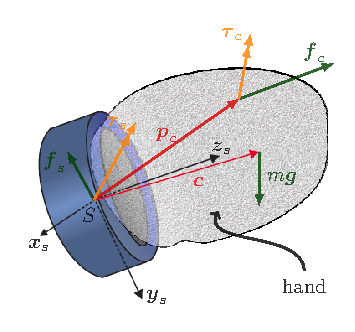
\includegraphics[width=\columnwidth]{ft_sensor_object}
    \end{column}
    \begin{column}{0.6\textwidth}
      \begin{itemize}
      \item[]-$\vec{f}_s$, -$\vec{\tau}_{s} :=$ measured forces
      \item[]-$\vec{f}_c$, -$\vec{\tau}_{c} :=$ contact forces 
      \item[] $\vec{f}_{pl}$, $\vec{\tau}_{pl} :=$ due to mounting plate \footnote[frame]{Not shown in the picture}
      \item[] $\vec{c} :=$ CoM of the hand
      \item[] $\vec{p}_c :=$ vector from $S$ to contact point
      \end{itemize}
    \end{column}
  \end{columns}
  \[
  \vec{w}_{S} = -
  \begin{bmatrix}
    \vec{f}_{c} \\
    \vec{\tau}_{c} +\tilde{\vec{p}}_{c} \vec{f}_{c}\\
  \end{bmatrix}
  \]
\end{frame}

\begin{frame}{Newton-Euler equations for a rigid body attached to the sensor}
  The Newton-Euler equations show how to obtain $\vec{w}_S$ from $\vec{f}_s$ and $\vec{\tau}_{s}$
  \[
  \vec{f}_{s} = - \vec{f}_{pl} - \alert{\vec{f}_{c}} -m  \vec{g} + m  \vec{a}_{cm}
  \]
  \[
  \vec{\tau}_{s}
  = - \vec{\tau}_{pl} - \alert{\vec{\tau}_{c}} - \tilde{\vec{p}}_{c}  \alert{\vec{f}_{c}}
  + \tilde{\vec{g}} m\vec{c} -  \tilde{\vec{a}}_{cm} m  \vec{c}
  \quad \footnote[frame]{Angular velocites and accelerations neglected because the f/t sensor
    is primarily used when the hand is still or when it moves along straight
    lines}
  \]
\end{frame}

\begin{frame}[shrink=20]{Software induced offset}
  The signal produced by the f/t sensor is
  \[
  \vec{f}_{meas} = -\vec{f}_{s} + \vec{f}_{sw,off}
  \]
  \[
  \vec{\tau}_{meas} = -\vec{\tau}_{s} + \vec{\tau}_{sw,off}
  \]
  Offsets $\vec{f}_{sw,off}$, $\vec{\tau}_{sw,off}$ are set when the f/t sensor is calibrated such that
  \[
  \vec{f}_{m,0} = \vec{\tau}_{m,0} = \vec{0}
  \footnote[frame]{The zero subscript represents the calbration condition performed
    when the manipulator is still}
  \]
  \[
  \vec{f}_{sw,off} = \vec{f}_{s,0} = -\vec{\tau}_{pl} -m \prescript{s}{}{ \vec{g}}_{0}
  \]
  \[
  \vec{\tau}_{sw,off} = \vec{\tau}_{s,0} = -\vec{\tau}_{pl} + \prescript{s}{}{ \tilde{\vec{g}}}_{0} m\vec{c}
  \]
  The resulting signal is
  \[
  \vec{f}_{meas} = \vec{f}_{c} +m \vec{g} -m \prescript{s}{}{ \vec{g}}_{0} - m  \vec{a}_{cm}
  \]
  \[
  \vec{\tau}_{meas} = \vec{\tau}_{c} + \tilde{\vec{p}}_{c}  \vec{f}_{c}
  - \tilde{\vec{g}} m\vec{c} + \prescript{s}{}{ \tilde{\vec{g}}}_{0} m\vec{c} +  \tilde{\vec{a}}_{cm} m  \vec{c}
  \]
\end{frame}

\begin{frame}[shrink=20]{Estimation of unknowns quantities}
  In order to obtain $\vec{f}_{c}$ and $\vec{\tau}_{c}$ the \alert{unkowns} are estimated
  \[
  \vec{f}_{meas} = \vec{f}_{c} +\alert{m} \vec{g} +(\alert{-m \prescript{s}{}{ \vec{g}}_{0}}) - m  \vec{a}_{cm}
  \]
  \[
  \vec{\tau}_{meas} = \vec{\tau}_{c} + \tilde{\vec{p}}_{c}  \vec{f}_{c}
  - \tilde{\vec{g}} \alert{m\vec{c}} + \alert{\prescript{s}{}{ \tilde{\vec{g}}}_{0} m\vec{c}} +  \tilde{\vec{a}}_{cm} \alert{m  \vec{c}}
  \]
  The estimation is obtained from $n$ measurements collected when the manipulator assumes a static pose
  \[
  \begin{bmatrix}
    \vec{f}_{meas} \\
    \vec{\tau}_{meas}
  \end{bmatrix} =
  \begin{bmatrix}
    \vec{g} m + (-m \prescript{s}{}{ \vec{g}}_{0}) \\
    -\tilde{\vec{g}} m\vec{c} + (\prescript{s}{}{ \tilde{\vec{g}}}_{0} m\vec{c})
  \end{bmatrix}
  =
  \begin{bmatrix}
    \vec{g} & 0_{3 \times 3} & I_{3x3} & 0_{3x3} \\
    \vec{0} & -\tilde{\vec{g}} & 0_{3x3} & I_{3x3}
  \end{bmatrix}
  \begin{bmatrix}
    m \\
    m \vec{c} \\
    -m \prescript{s}{}{ \vec{g}}_{0} \\
    \prescript{s}{}{ \tilde{\vec{g}}}_{0} m\vec{c}
  \end{bmatrix}
  =
  H(\prescript{s}{}{\vec{g}(\vec{q})}) \vec{\theta}
  =
  H(\vec{q}) \vec{\theta}
  \]
  \[
  \begin{split}
    \hat{\vec{\theta}} &=
    \begin{bmatrix}
      H(\vec{q}^{1})\\
      \vdots \\
      H(\vec{q}^{n})\\
    \end{bmatrix}^{+}
    \begin{bmatrix}
      \vec{f}_{m}^{1} \\
      \vec{\tau}_{m}^{1} \\
      \vdots \\
      \vec{f}_{m}^{n} \\
      \vec{\tau}_{m}^{n} \\
    \end{bmatrix}
    =
    H_n^{+}
    \begin{bmatrix}
      \vec{f}_{m}^{1} \\
      \vec{\tau}_{m}^{1} \\
      \vdots \\
      \vec{f}_{m}^{n} \\
      \vec{\tau}_{m}^{n} \\
    \end{bmatrix}\\
  \end{split}
  \]
\end{frame}

\begin{frame}{Estimation of unknowns quantities - An example}
  \vskip0.1in
  \begin{columns}
    \begin{column}{0.5\textwidth}
      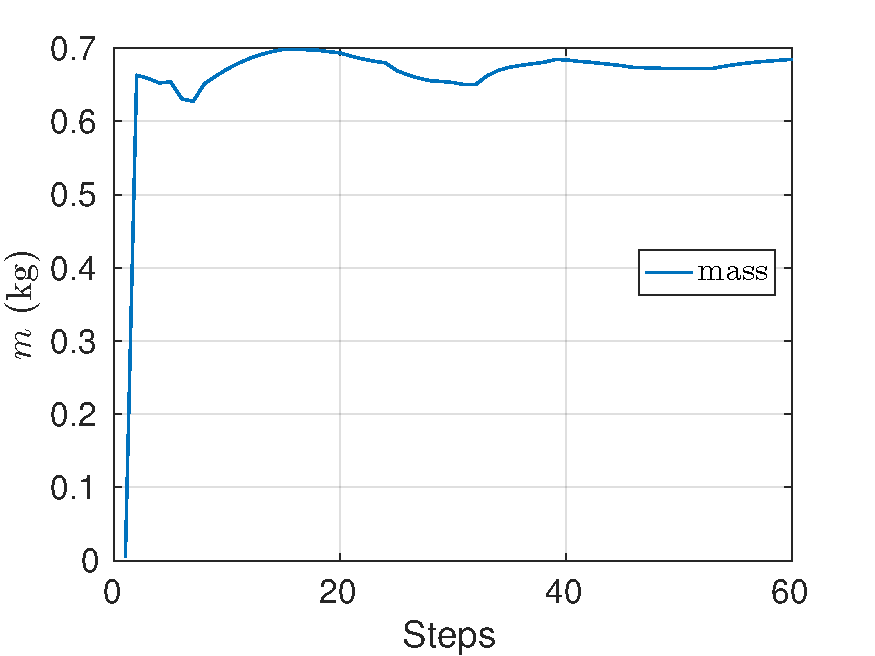
\includegraphics[width=\columnwidth]{mass}\\
      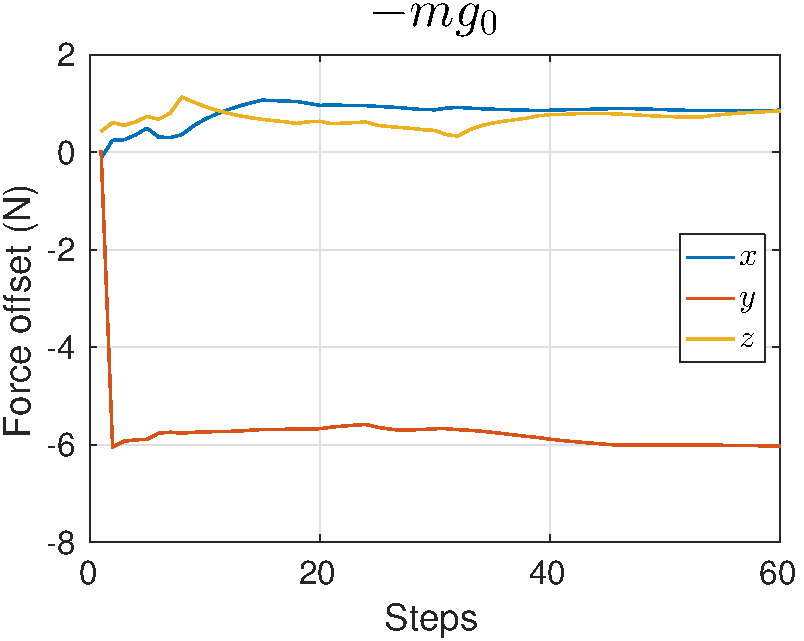
\includegraphics[width=\columnwidth]{off_f}
    \end{column}
    \begin{column}{0.5\textwidth}
      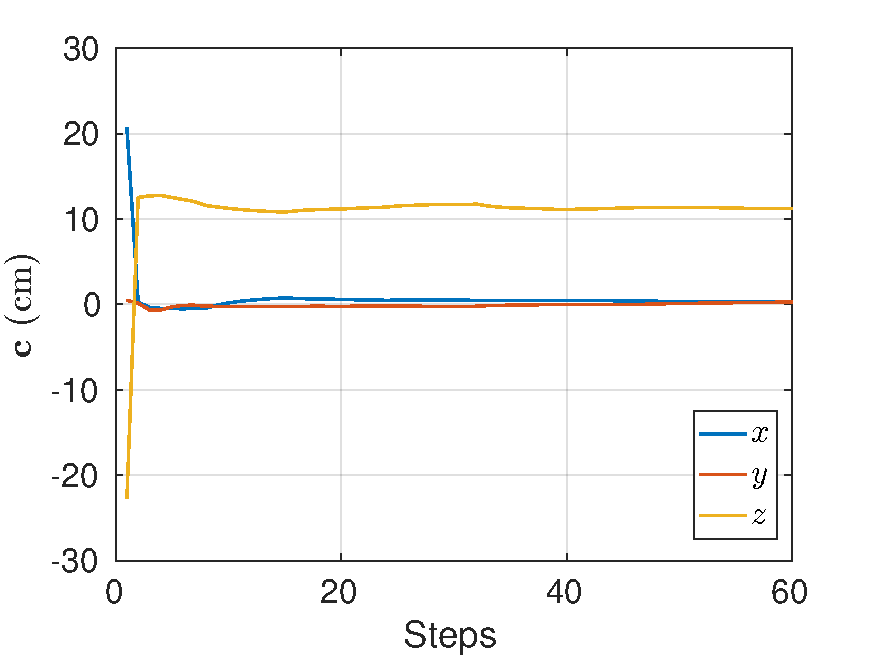
\includegraphics[width=\columnwidth]{com}\\
      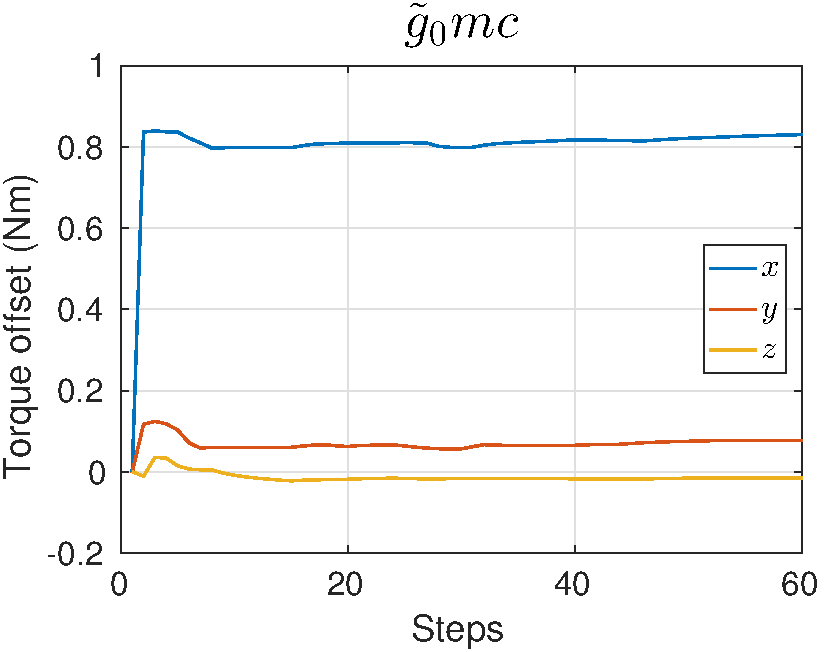
\includegraphics[width=\columnwidth]{off_t}
    \end{column}
  \end{columns}
\end{frame}

